% ============================================================
%  File: Chapter9.tex
%  \input this file as a chapter.
%  All environments reference the existing preamble; no extra
%  \usepackage or \definecolor declarations are needed.
% ============================================================

% ── Local TikZ styles ────────────────────────────────────────
\tikzset{
	slkblock/.style={
		rectangle, rounded corners=4pt,
		draw=blue!60!black, fill=blue!8,
		text width=#1, minimum height=1.0cm,
		align=center, font=\small\bfseries\sffamily
	},
	slkblock/.default=2.8cm,
	slkgreen/.style={slkblock=#1, draw=teal, fill=green!8},
	slkgreen/.default=2.8cm,
	slkred/.style={slkblock=#1, draw=red!70!black, fill=red!6},
	slkred/.default=2.8cm,
	slkyellow/.style={slkblock=#1, draw=yellow!60!black, fill=yellow!10},
	slkyellow/.default=2.8cm,
	slkarrow/.style={-Stealth, thick, draw=blue!60!black},
	slkdarrow/.style={-Stealth, thick, dashed, draw=red!60!black},
	siglabel/.style={font=\scriptsize\sffamily\itshape, midway},
	siglabelabove/.style={siglabel, above},
	siglabelbelow/.style={siglabel, below},
	siglabelright/.style={siglabel, right},
	siglabelleft/.style={siglabel, left},
}

% ============================================================
\chapter{Simulink Implementation of Model Predictive Control\texorpdfstring{$^{(*)}$}{(*)}}
\label{chap:simulink_mpc}
% ============================================================

% ─────────────────────────────────────────────────────────────
\section{General Implementation Guidance}
\label{sec:simulink_general}
% ─────────────────────────────────────────────────────────────

Simulink is widely used for rapid prototyping and hardware-in-the-loop
validation of control systems, and Model Predictive Control (MPC) is no
exception.  Implementing MPC in Simulink without the dedicated MPC
Toolbox requires a careful architectural decision: the optimisation
solver must be invoked at every simulation time step from within a
Simulink block, yet the solver itself — together with the YALMIP
modelling layer — relies on dynamic MATLAB features that are
incompatible with Simulink's default code-generation pipeline.  This
section establishes a general framework that resolves this tension.  The
approach is first described in fully general terms; Section~\ref{sec:simulink_building}
then applies it step by step to a concrete building temperature control
system.

% ─────────────────────────────────────────────────────────────
\subsection{Why the MPC Toolbox Is Not Required}
\label{subsec:no_toolbox}
% ─────────────────────────────────────────────────────────────

The MathWorks MPC Toolbox offers convenient pre-built blocks but
abstracts away the optimisation layer entirely.  This abstraction
becomes a limitation whenever the designer requires any of the
following:

\begin{itemize}[noitemsep]
	\item \textbf{Economic (non-regulatory) objectives} — for instance,
	minimising energy cost rather than a quadratic deviation from a
	setpoint;
	\item \textbf{Augmented observers} — such as Kalman filters that
	jointly estimate the plant state and an unmeasured disturbance;
	\item \textbf{Time-varying constraints} — comfort bands or
	operational limits that change according to a schedule;
	\item \textbf{Custom terminal costs or terminal sets} — required for
	rigorous closed-loop stability guarantees.
\end{itemize}

Using YALMIP together with \texttt{quadprog} or OSQP provides all of
this flexibility whilst keeping solver call-time well within a typical
sampling period.

% ─────────────────────────────────────────────────────────────
\subsection{The Code-Generation Barrier and How to Overcome It}
\label{subsec:extrinsic}
% ─────────────────────────────────────────────────────────────

MATLAB Function blocks in Simulink normally compile their contents into
C code at simulation start.  YALMIP relies on dynamic cell arrays,
runtime type inspection, and variable-argument function calls — none of
which survive compilation.  Attempting to call \texttt{sdpvar},
\texttt{optimizer}, or any YALMIP routine directly inside a compiled
block produces an immediate error.

The standard remedy is the \texttt{coder.extrinsic} declaration.  Any
function declared as extrinsic is \emph{not} compiled; instead, it
executes inside the full MATLAB interpreter at run time.  The
simulation still advances correctly — the block simply runs in
interpreted mode for the declared functions.

\begin{notebox}{Rules for \texttt{coder.extrinsic}}
	\begin{enumerate}[noitemsep]
		\item The declaration must appear at the \emph{top} of the MATLAB
		Function block body, before any use of the function.
		\item Every output variable must be \emph{pre-allocated} to a
		concrete type and size before the extrinsic call, so that
		Simulink can infer port dimensions at compile time.
		\item All YALMIP-dependent logic should live in a separate
		\texttt{.m} helper file; the block itself contains only the
		declaration and a single forwarding call.
	\end{enumerate}
	
	The general pattern inside any MATLAB Function block is:
	
	\begin{lstlisting}[language=Matlab]
		function y = MyBlock(u)
			coder.extrinsic('my_helper');   % declare before use
			y = zeros(size_of_output);      % pre-allocate
			y = my_helper(u);               % forward to helper
		end
	\end{lstlisting}
\end{notebox}

% ─────────────────────────────────────────────────────────────
\subsection{Managing State Across Time Steps: Persistent Variables}
\label{subsec:persistent}
% ─────────────────────────────────────────────────────────────

A Simulink MATLAB Function block does not retain values in its
workspace between consecutive invocations — each call begins with a
clean local scope.  An MPC controller, however, must preserve several
quantities across every time step:

\begin{itemize}[noitemsep]
	\item the observer state estimate $\hat{z}_k$;
	\item the last applied input $u_{k-1}$ (needed for the observer
	prediction step);
	\item any filtered disturbance estimates;
	\item the compiled YALMIP \texttt{optimizer} objects.
\end{itemize}

MATLAB's \texttt{persistent} keyword solves this problem.  A
persistent variable is initialised once on the first function call
and retains its value for the lifetime of the function in memory.
Within a Simulink simulation, this means the variable persists across
every time step from $k=1$ to the end of the run.

\begin{defnbox}{Persistent Variable Pattern for MPC Helper Functions}
	Declare all cross-step quantities with \texttt{persistent} at the
	top of the helper \texttt{.m} file, then guard initialisation with
	an \texttt{isempty} check:
	
	\begin{lstlisting}[language=Matlab]
		function u = my_mpc_step(y_meas, ...)
			persistent opt_obj observer_state u_prev
		
			if isempty(observer_state)           % runs on first call only
				opt_obj        = build_optimizers();
				observer_state = x0_guess;
				u_prev         = 0;
			end
		
			% ... rest of the control pipeline ...
		end
	\end{lstlisting}
	
	\textbf{Important:} before starting a new simulation run always
	execute \texttt{clear \textit{functionname}} in the MATLAB Command
	Window.  This resets all persistent variables to their initial
	state; failure to do so causes the controller to inherit the
	terminal conditions of the previous run.
\end{defnbox}

% ─────────────────────────────────────────────────────────────
\subsection{Building YALMIP Optimiser Objects: One-Time Compilation}
\label{subsec:build_general}
% ─────────────────────────────────────────────────────────────

YALMIP's \texttt{optimizer} function pre-processes the problem
structure — symbolic variable registration, sparsity analysis, and
conversion to the solver's native QP format — and returns a compiled
function handle.  This pre-processing is the expensive step (typically
10--30\,s for moderate-sized problems) and must not be repeated at
every simulation time step.

The correct approach is to create a dedicated initialisation function,
call it exactly once inside the persistent-variable guard shown above,
and store the resulting objects as persistent variables.  All
subsequent time steps call the compiled objects directly, which
typically completes in milliseconds.

\begin{lstlisting}[language=Matlab, caption={Skeleton of a one-time YALMIP initialisation function.}]
	function [opt1, opt2] = build_optimizers()
		% Called once. Returns compiled optimizer objects.
	
		% -- Define symbolic decision variables -----------------------
		x  = sdpvar(nx, 1);
		u  = sdpvar(nu, 1);
		p  = sdpvar(np, 1);    % parametric inputs (e.g. price, bounds)
	
		% -- Formulate constraints and objective ----------------------
		con = [ ... ];         % linear/quadratic constraints
		obj = ... ;            % quadratic cost
	
		% -- Compile with chosen solver -------------------------------
		ops  = sdpsettings('solver', 'quadprog', 'verbose', 0);
		opt1 = optimizer(con, obj, ops, {p}, {u});
	
		% -- Second optimizer (e.g. target calculator) ----------------
		% ...
	end
\end{lstlisting}

% ─────────────────────────────────────────────────────────────
\subsection{Recommended Architecture}
\label{subsec:architecture}
% ─────────────────────────────────────────────────────────────

The architecture that best reconciles Simulink's execution model with
YALMIP's requirements separates the design into two layers, as shown in
Figure~\ref{fig:architecture}.

\emph{Layer 1 — the Simulink canvas} contains only standard Simulink
blocks and thin MATLAB Function wrapper blocks.  Each wrapper declares
one helper function as extrinsic, pre-allocates its outputs, and
forwards its inputs.  Signal routing, the feedback connection, noise
injection, and input saturation are all handled by built-in Simulink
blocks.

\emph{Layer 2 — the helper \texttt{.m} files} contain all
computation: observer updates, YALMIP calls, QP solves, and persistent
state.  Because they execute in the full MATLAB interpreter they impose
no restrictions on the code they contain.

\begin{figure}[htbp]
	\centering
	\resizebox{\textwidth}{!}{%
		\begin{tikzpicture}[node distance=0.9cm and 3.2cm]
			
			%% ── Simulink layer: left column ──
			\node[slkyellow=3.4cm] (distgen)
			{Exogenous Signal\\Generator\\MATLAB Fn block};
			
			\node[slkblock=3.4cm, below=0.8cm of distgen] (plant)
			{Plant\\MATLAB Fn block};
			
			\node[slkblock=3.4cm, below=0.8cm of plant] (noise)
			{Measurement Noise\\{\scriptsize Sum + Random Number}};
			
			\node[slkblock=3.4cm, below=0.8cm of noise] (ctrl)
			{MPC Controller\\MATLAB Fn block};
			
			\node[slkblock=3.4cm, below=0.8cm of ctrl] (sat)
			{Saturation\\$[u_{\min},\;u_{\max}]$};
			
			%% ── Helper layer: right column ──
			\node[slkgreen=4.8cm, right=3.4cm of distgen] (hgen)
			{\texttt{signal\_generator.m}\\[2pt]
				{\small\normalfont Returns disturbances, references,\\
					and constraint parameters}};
			
			\node[slkgreen=4.8cm, right=3.4cm of plant] (hplant)
			{\texttt{plant\_model.m}\\[2pt]
				{\small\normalfont Discrete-time state update;\\
					persistent true state \texttt{x\_true}}};
			
			\node[slkgreen=4.8cm, right=3.4cm of ctrl] (hctrl)
			{\texttt{mpc\_step.m}\\[2pt]
				{\small\normalfont Observer update, target calculation,\\
					MPC QP solve; all persistent state}};
			
			\node[slkyellow=4.8cm, below=1.0cm of hctrl] (hbuild)
			{\texttt{build\_optimizers.m}\\[2pt]
				{\small\normalfont Builds YALMIP \texttt{optimizer} objects\\
					and observer gain; called once only}};
			
			%% ── Bounding boxes ──
			\begin{scope}[on background layer]
				\node[draw=blue!50, fill=blue!4, rounded corners=8pt,
				fit=(distgen)(plant)(noise)(ctrl)(sat),
				inner sep=12pt,
				label={[font=\small\bfseries\sffamily\color{blue!60!black}]
					above:{Layer 1 --- Simulink Canvas}}]
				(simbox) {};
			\end{scope}
			\begin{scope}[on background layer]
				\node[draw=teal, fill=green!4, rounded corners=8pt,
				fit=(hgen)(hplant)(hctrl)(hbuild),
				inner sep=12pt,
				label={[font=\small\bfseries\sffamily\color{teal}]
					above:{Layer 2 --- Helper \texttt{.m} Files (MATLAB Path)}}]
				(helperbox) {};
			\end{scope}
			
			%% ── Extrinsic call arrows ──
			\draw[slkarrow] (distgen.east) --
			node[siglabelabove]{\texttt{coder.extrinsic}} (hgen.west);
			\draw[slkarrow] (plant.east) --
			node[siglabelabove]{\texttt{coder.extrinsic}} (hplant.west);
			\draw[slkarrow] (ctrl.east) --
			node[siglabelabove]{\texttt{coder.extrinsic}} (hctrl.west);
			
			%% ── One-time build call (dashed) ──
			\draw[slkdarrow] (hctrl.south) --
			node[siglabelright, align=left]{called once\\(persistent guard)}
			(hbuild.north);
			
			%% ── Vertical signal flow within Simulink ──
			\draw[slkarrow] (distgen.south) --
			node[siglabelright]{$d_k$,\; known inputs} (plant.north);
			\draw[slkarrow] (plant.south) --
			node[siglabelright]{$y_\mathrm{true}$} (noise.north);
			\draw[slkarrow] (noise.south) --
			node[siglabelright]{$y_\mathrm{meas}$} (ctrl.north);
			\draw[slkarrow] (ctrl.south) --
			node[siglabelright]{$u_\mathrm{raw}$} (sat.north);
			
			%% ── Feedforward: exogenous signals to controller ──
			%% Four-leg orthogonal route: left → down → right → down into ctrl.west
			\coordinate (ffTurn)    at ($(distgen.west) + (-1.0, 0)$);
			\coordinate (ffApproach) at ($(ctrl.west)   + (-1.0, 0)$);
			
\draw[slkarrow]
(distgen.west)
-- (ffTurn)
-- (ffTurn |- ffApproach)
-- node[siglabelleft, align=left]{$r_k$\\exogenous inputs\\constraint parameters}
(ffApproach)
-- (ctrl.west);
			
			%% ── Feedback: Unit Delay ──
			\coordinate (fbTurn)   at ($(sat.west)  + (-1.8, 0)$);
			\coordinate (fbTarget) at ($(plant.west)+ (-1.8, 0)$);
			
			\draw[slkarrow]
			(sat.west)
			-- (fbTurn)                        % 1. left of sat
			-- (fbTarget)                      % 2. up alongside left edge
			-- node[siglabelabove]{$u_{k-1}$\; (Unit Delay)}
			([yshift=0pt]plant.west);       % 3. right into plant
			
		\end{tikzpicture}%
	}
	\caption{General two-layer architecture for Simulink-based MPC without the
		MPC Toolbox.  Layer~1 (Simulink canvas) contains only thin MATLAB Function
		wrapper blocks; all optimisation logic is delegated to Layer~2 helper files
		via \texttt{coder.extrinsic} calls.  Persistent variables in the helper files
		carry state across time steps and store the compiled \texttt{optimizer}
		objects for the lifetime of the simulation.}
	\label{fig:architecture}
\end{figure}

% ─────────────────────────────────────────────────────────────
\subsection{Eliminating the Algebraic Loop}
\label{subsec:algloop_general}
% ─────────────────────────────────────────────────────────────

In any discrete-time closed-loop Simulink model of the form
Plant~$\to$~Controller~$\to$~Plant, Simulink detects an
\emph{algebraic loop}: computing the plant output $y_k$ requires
the current input $u_k$, which itself requires $y_k$.  The standard
remedy is to insert a \emph{Unit Delay} block between the controller
output (or the saturation block) and the plant input:

\[
\cdots \to \text{Saturation} \;\xrightarrow{\;u_k\;}\;
\underbrace{\text{Unit Delay}}_{T_s,\;\mathrm{IC}=0}
\;\xrightarrow{\;u_{k-1}\;}\; \text{Plant} \to \cdots
\]

This is not an approximation — in a physically realisable digital
controller the input computed at step~$k$ cannot reach the actuator
until step~$k{+}1$.  The observer in the MPC helper file must
therefore use $u_{k-1}$ (stored as a persistent variable) rather than
$u_k$ in its prediction equation, which is achieved automatically by
the pattern shown in Section~\ref{subsec:persistent}.

% ─────────────────────────────────────────────────────────────
\subsection{Solver Recommendations}
\label{subsec:solvers}
% ─────────────────────────────────────────────────────────────

YALMIP supports a wide range of QP solvers through a common interface.
For typical MPC problems — moderate-horizon quadratic programmes with
linear constraints — the following two solvers are recommended.

\begin{center}
	\begin{tabular}{>{\bfseries\sffamily}l p{4.2cm} p{5.6cm}}
		\toprule
		Solver & Availability & Notes \\
		\midrule
		\texttt{quadprog} &
		Ships with MATLAB Optimisation Toolbox &
		Reliable, no warm-start across calls; sufficient for $N \leq 30$ \\[4pt]
		OSQP &
		Free, open-source; install via \texttt{osqp-matlab} &
		Supports warm-starting; recommended for long horizons or fast
		sampling rates \\
		\bottomrule
	\end{tabular}
\end{center}

Both are specified in YALMIP identically:
\begin{center}
\texttt{sdpsettings('solver','quadprog',...)} 
\end{center}


or
\begin{center}
\texttt{sdpsettings('solver','osqp',...)}.
\end{center}


% ─────────────────────────────────────────────────────────────
\subsection{Summary of the Implementation Workflow}
\label{subsec:workflow_summary}
% ─────────────────────────────────────────────────────────────

Figure~\ref{fig:workflow} summarises the complete development workflow.
The left column shows the \emph{offline} design steps that are
completed once before the Simulink model is built.  The right column
shows the \emph{runtime} sequence that executes automatically during
simulation.

\begin{figure}[htbp]
	\centering
	\resizebox{0.82\textwidth}{!}{%
		\begin{tikzpicture}[node distance=0.5cm]
			
			% ── OFFLINE column ──
			\node[slkblock=4.2cm] (d1) {Design discrete-time plant model \& choose $T_s$};
			\node[slkblock=4.2cm, below=0.5cm of d1] (d2) {Design observer\\(e.g.\ augmented Kalman filter)};
			\node[slkblock=4.2cm, below=0.5cm of d2] (d3) {Formulate YALMIP\\\texttt{optimizer} objects\\(cost, constraints, horizon)};
			\node[slkblock=4.2cm, below=0.5cm of d3] (d4) {Write helper \texttt{.m} files:\\
				\texttt{build\_optimizers.m},\\
				\texttt{plant\_model.m},\\
				\texttt{mpc\_step.m}, \ldots};
			\node[slkblock=4.2cm, below=0.5cm of d4] (d5) {Build Simulink model:\\
				add blocks, set solver to\\
				fixed-step discrete, $T_s$};
			
			\draw[slkarrow] (d1)--(d2); \draw[slkarrow] (d2)--(d3);
			\draw[slkarrow] (d3)--(d4); \draw[slkarrow] (d4)--(d5);
			
			\begin{scope}[on background layer]
				\node[draw=blue!50, fill=blue!4, rounded corners=6pt,
				fit=(d1)(d2)(d3)(d4)(d5), inner sep=10pt,
				label={[font=\small\bfseries\sffamily\color{blue!60!black}]
					above:Offline Design}] {};
			\end{scope}
			
			% ── RUNTIME column ──
			\node[slkgreen=4.2cm, right=2.8cm of d1] (r1)
			{\texttt{clear plant\_model}\\
				\texttt{clear mpc\_step}\\
				{\small(reset persistent vars)}};
			\node[slkgreen=4.2cm, below=0.5cm of r1] (r2)
			{Step $k=1$: \texttt{isempty} guard\\calls \texttt{build\_optimizers};\\
				YALMIP compiles QPs};
			\node[slkgreen=4.2cm, below=0.5cm of r2] (r3)
			{Steps $k \geq 2$:\\
				observer predict \& correct\\
				$\rightarrow$ target solve\\
				$\rightarrow$ MPC QP solve};
			\node[slkgreen=4.2cm, below=0.5cm of r3] (r4)
			{Apply $u_k$; Unit Delay\\feeds $u_{k-1}$ to plant\\at step $k{+}1$};
			\node[slkyellow=4.2cm, below=0.5cm of r4] (r5)
			{Simulation ends;\\ post-process logged signals};
			
			\draw[slkarrow] (r1)--(r2); \draw[slkarrow] (r2)--(r3);
			\draw[slkarrow] (r3)--(r4); \draw[slkarrow] (r4.east) -- ++(0.5,0) -- ++(0,1.5) -- node[siglabelright]{repeat $\forall k$} ++(-0.5,0)
			node[siglabelright]{repeat $\forall k$} (r3);
			\draw[slkarrow] (r4)--(r5);
			
			\begin{scope}[on background layer]
				\node[draw=teal, fill=green!4, rounded corners=6pt,
				fit=(r1)(r2)(r3)(r4)(r5), inner sep=10pt,
				label={[font=\small\bfseries\sffamily\color{teal}]
					above:Simulation Runtime}] {};
			\end{scope}
			
		\coordinate (mid) at ($(d5.east)!0.5!(r1.west)$);  % halfway horizontally
		
		\draw[slkarrow, ultra thick]
		(d5.east)
		-- (mid |- d5.east)                   % 1. right → midpoint, same height as d5
		-- (mid |- r1.west)                   % 2. up   → midpoint, same height as r1
		-- (r1.west)                          % 3. right → r1
		node[above, font=\small\sffamily, pos=0.5]{run};
			
		\end{tikzpicture}%
	}
	\caption{Complete Simulink MPC development and execution workflow.  The
		offline design phase (left) produces all \texttt{.m} helper files and
		the Simulink model.  On each new simulation run the persistent
		variables are cleared manually, after which the runtime sequence
		(right) executes automatically, compiling YALMIP objects once on the
		first step and solving the QP at every subsequent step.}
	\label{fig:workflow}
\end{figure}

% =============================================================

\section{Case Study: Single-Zone Building Heating}
\label{sec:simulink_building}
% =============================================================

We revisit the single-zone office heating problem introduced in the
previous chapter.  The general framework of
Section~\ref{sec:simulink_general} is now applied step by step to the
three-state physically derived RC model, combining an augmented Kalman
filter — which jointly estimates the three thermal states and an
unmeasured occupancy disturbance — with a two-layer economic MPC
comprising an economic steady-state target calculator and a
deviation-form MPC regulator with electricity-price preview.  This
example exercises every aspect of the general framework: persistent
optimiser objects, a multi-output profile generator, an extrinsic plant
block, and a feedback loop broken by a Unit Delay.

% -----------------------------------------------------------------
\subsection{System Description}
\label{subsec:system}
% -----------------------------------------------------------------

The discrete-time model of the single-zone building (sampling period
$T_s = 1800\,\mathrm{s}$, i.e.\ 30~min) is

\begin{equation*}
	x_{k+1} = A x_k + B u_k + E\,T_{\mathrm{amb},k}
	+ B_{\mathrm{sol}}\,\varphi_{\mathrm{sol},k}
	+ B_w\,d_k,
	\qquad
	y_k = C x_k + v_k,
\end{equation*}

\noindent where
$x_k = [T_{\mathrm{air},k},\; T_{w,\mathrm{in},k},\; T_{w,\mathrm{out},k}]^\top
\in \mathbb{R}^3$
contains indoor air temperature and the two wall-layer temperatures,
$u_k \in [0,\,2000]\,\mathrm{W}$ is heater power,
$T_{\mathrm{amb},k}$ and $\varphi_{\mathrm{sol},k}$ are the
\emph{measured} outdoor temperature and solar irradiance (known
feedforwards), and $d_k$ (${}^\circ$C/step) is the
\emph{unmeasured} occupancy-driven thermal disturbance.  The output

\[
y_k = 0.56\,T_{\mathrm{air},k} + 0.44\,T_{w,\mathrm{in},k}
\]

is the operative temperature (ISO~7726), measured with noise standard
deviation $\sigma_v = 0.1\,{}^\circ$C.

The pre-computed ZOH-discretised matrices are
\begin{multline*}
	A = \begin{bmatrix}
		0.8753 & 0.1102 & 0.0004 \\
		0.0275 & 0.9649 & 0.0073 \\
		0.0001 & 0.0049 & 0.9851
	\end{bmatrix}, \quad
	B = \begin{bmatrix}7.91\times10^{-4}\\1.00\times10^{-4}\\0\end{bmatrix},\quad
	E  = \begin{bmatrix}0.01404\\0.00025\\0.00993\end{bmatrix},\\[4pt]
	B_{\mathrm{sol}} = \begin{bmatrix}9.04\times10^{-6}\\1.43\times10^{-6}\\3.47\times10^{-4}\end{bmatrix}, \quad
	B_w = \begin{bmatrix}1.7647\\0.0267\\0\end{bmatrix},\quad
	C  = \begin{bmatrix}0.56 & 0.44 & 0\end{bmatrix}.
\end{multline*}

The control objective is to minimise electricity cost subject to
comfort constraints:
\[
y_{\min,k} \;\leq\; y_k \;\leq\; y_{\max,k},
\qquad
0 \;\leq\; u_k \;\leq\; 2000\,\mathrm{W},
\]
where the comfort bounds follow a daily occupancy schedule
($[20,\,23]\,{}^\circ$C during occupied hours 07:00--22:00,
$[15,\,26]\,{}^\circ$C overnight).

% -----------------------------------------------------------------
\subsection{File Structure}
\label{subsec:filestructure}
% -----------------------------------------------------------------

Following the general architecture of Section~\ref{subsec:architecture},
the implementation consists of four helper \texttt{.m} files and one
Simulink model file.  Table~\ref{tab:files} maps each file to the
corresponding generic role.

\begin{table}[htbp]
	\centering
	\caption{Helper files for the single-zone building case study and their
		correspondence to the general architecture.}
	\label{tab:files}
	\begin{tabular}{>{\ttfamily\small}l >{\small}l >{\small}p{5.2cm}}
		\toprule
		\normalfont\textbf{File} & \textbf{Generic role} & \textbf{Purpose} \\
		\midrule
		build\_mpc\_optimizers.m & \texttt{build\_optimizers.m} &
		Kalman gain (DARE), economic target \texttt{optimizer}, MPC regulator
		\texttt{optimizer} with price preview; called once \\[4pt]
		get\_profiles.m & \texttt{disturbance\_profiles.m} &
		Ambient temperature, solar irradiance, electricity price, current
		comfort bounds, and $N$-step future comfort bound vectors \\[4pt]
		plant\_step.m & \texttt{plant\_model.m} &
		One-step advance of the discrete RC building model; persistent
		true state \texttt{x\_true} and true occupancy disturbance \\[4pt]
		mpc\_controller\_step.m & \texttt{mpc\_step.m} &
		Kalman observer, economic target calculation, economic MPC QP
		solve with price preview; all state persistent \\[4pt]
		EconomicMPC.slx & Simulink model &
		Wires all wrapper blocks and standard blocks together \\
		\bottomrule
	\end{tabular}
\end{table}

All \texttt{.m} files and \texttt{EconomicMPC.slx} must reside in the
same folder, or all \texttt{.m} files must be accessible via
\texttt{addpath}.

% -----------------------------------------------------------------
\subsection{Step 1 — \texttt{build\_mpc\_optimizers.m}}
\label{subsec:build}
% -----------------------------------------------------------------

This function fulfils the role of the generic \texttt{build\_optimizers.m}
described in Section~\ref{subsec:build_general}.  It computes the
steady-state Kalman gain via \texttt{dare} and pre-compiles two YALMIP
\texttt{optimizer} objects: one for the economic steady-state target
and one for the deviation-form MPC regulator with $N$-step price
preview.  The compilation step runs exactly once, since the resulting
objects are stored as persistent variables in
\texttt{mpc\_controller\_step.m}.

\begin{lstlisting}[language=Matlab,
	caption={\texttt{build\_mpc\_optimizers.m} --- one-time initialisation
		function for the single-zone building controller.},
	label={lst:build}]
	function [target_calc, mpc_reg, L] = build_mpc_optimizers()
		% Builds YALMIP optimizer objects and the Kalman gain.
		% Called exactly once via the persistent guard in mpc_controller_step.m.
		fprintf('Building YALMIP optimizers -- please wait...\n');
		
		Ts = 1800;
		A     = [0.8753, 0.1102, 0.0004;
					0.0275, 0.9649, 0.0073;
					0.0001, 0.0049, 0.9851];
		B     = [7.91e-4; 1.00e-4; 0      ];
		E     = [0.01404; 0.00025; 0.00993];
		Bsol  = [9.04e-6; 1.43e-6; 3.47e-4];
		Bw    = [1.7647;  0.0267;  0      ];
		C     =  [0.56, 0.44, 0];
		nx = 3;  nu = 1;  u_min = 0;  u_max = 2000;
		
		%% -- Augmented Kalman filter (state + occupancy disturbance) ------
		%    z = [x; d],  random-walk disturbance model
		A_aug   = [A, Bw; zeros(1,nx), 1];
		B_aug   = [B; 0];
		E_aug   = [E; 0];
		Bsol_aug= [Bsol; 0];
		C_aug   = [C, 0];
		
		W_kf = diag([1e-3, 1e-3, 1e-3, (0.01)^2]);  % sqrt(W_d)=0.01 degC/step
		V_kf = 0.1^2;
		[P_kf,~,~] = dare(A_aug', C_aug', W_kf, V_kf);
		L = P_kf * C_aug' / (C_aug * P_kf * C_aug' + V_kf);
		
		%% -- Economic steady-state target optimizer -----------------------
		price_k  = sdpvar(1,1);  d_hat_k  = sdpvar(1,1);
		T_amb_k  = sdpvar(1,1);  phi_k    = sdpvar(1,1);
		y_min_k  = sdpvar(1,1);  y_max_k  = sdpvar(1,1);
		xs = sdpvar(nx,1);  us = sdpvar(nu,1);  ss_slack = sdpvar(1,1);
		
		ss_cons = [xs == A*xs + B*us + E*T_amb_k + Bsol*phi_k + Bw*d_hat_k, ...
		y_min_k - ss_slack <= C*xs <= y_max_k + ss_slack, ...
		u_min <= us <= u_max,  ss_slack >= 0];
		ss_obj  = price_k * us + 1e4 * ss_slack^2;
		
		ops_ss      = sdpsettings('solver','quadprog','verbose',0);
		target_calc = optimizer(ss_cons, ss_obj, ops_ss, ...
		{price_k, d_hat_k, T_amb_k, phi_k, y_min_k, y_max_k}, ...
		[xs; us]);
		
		%% -- Economic MPC regulator with N-step price preview -------------
		%    Stage cost: ||x_tilde||_Q^2 + beta*price*u*(Ts/3600) + rho*slack^2
		%    Penalty hierarchy: rho >> beta*p_max*u_max*(Ts/3600)
		%    i.e.  1e7 >> 6*0.28*2000*0.5 = 1680
		N = 24;  Q = diag([5,2,1]);  beta = 6;  rho = 1e7;
		[P_term,~,~] = dare(A, B, Q, 1e-3);
		
		du_v     = sdpvar(nu,N,'full');    dx_v  = sdpvar(nx,N+1,'full');
		slk      = sdpvar(1,N,'full');
		xh_v     = sdpvar(nx,1);   xs_v = sdpvar(nx,1);  us_v = sdpvar(nu,1);
		Ymn      = sdpvar(1,N,'full');     Ymx   = sdpvar(1,N,'full');
		Price_v  = sdpvar(1,N,'full');
		
		obj = 0;
		con = [dx_v(:,1) == xh_v - xs_v];
		for i = 1:N
			u_abs = du_v(:,i) + us_v;
			x_pred_i = dx_v(:,i+1) + xs_v;
			con = [con, ...
			dx_v(:,i+1) == A*dx_v(:,i) + B*du_v(:,i), ...
			u_min <= u_abs <= u_max, ...
			Ymn(i)-slk(i) <= C*x_pred_i <= Ymx(i)+slk(i), slk(i) >= 0];
			obj = obj + dx_v(:,i)'*Q*dx_v(:,i) ...
			+ beta*Price_v(i)*u_abs*(Ts/3600) ...
			+ rho*slk(i)^2;
		end
		obj = obj + dx_v(:,N+1)' * P_term * dx_v(:,N+1);
		
		ops_mpc = sdpsettings('solver','quadprog','verbose',0);
		mpc_reg = optimizer(con, obj, ops_mpc, ...
		{xh_v, xs_v, us_v, Ymn, Ymx, Price_v}, du_v(:,1));
		
		fprintf('Optimizers ready.\n');
	end
\end{lstlisting}

\begin{notebox}{Horizon and Tuning Parameters}
	The prediction horizon $N = 24$ steps corresponds to 12\,hours at
	$T_s = 30\,\mathrm{min}$, allowing the controller to anticipate the
	morning and evening price transitions.  The state penalty
	$Q = \mathrm{diag}(5,2,1)$ weights the air temperature most heavily.
	The economic weight $\beta = 6$ and the comfort slack penalty
	$\rho = 10^7$ satisfy the hierarchy $\rho \gg
	\beta\,p_{\max}\,u_{\max}\,(T_s/3600) = 1680$, guaranteeing that
	comfort violations are never preferred over heating.  The terminal
	cost $P_\infty$ is the DARE solution, ensuring asymptotic stability
	of the unconstrained closed-loop.
\end{notebox}

% -----------------------------------------------------------------
\subsection{Step 2 — \texttt{get\_profiles.m}}
\label{subsec:profiles}
% -----------------------------------------------------------------

This function fulfils the role of the generic
\texttt{disturbance\_profiles.m}.  It receives the current simulation
time in seconds from the Simulink \textit{Clock} block and returns all
time-varying exogenous signals: ambient temperature, solar irradiance,
electricity price, current comfort bounds, and the $N$-step future
comfort bound and price vectors required by the MPC optimiser.

\begin{lstlisting}[language=Matlab,
	caption={\texttt{get\_profiles.m} --- provides current and forecast
		exogenous signals for the MPC horizon (48-hour winter scenario).},
	label={lst:profiles}]
	function [T_amb, Solar, Price, Tmin, Tmax, Tmin_fut, Tmax_fut, Price_fut] = ...
	get_profiles(t)
		% Input:  t in seconds (Simulink Clock output).
		% Outputs: scalars for current step + 1x24 vectors for MPC horizon.
		N  = 24;  Ts = 1800;  t_h = t / 3600;
		
		% Outdoor temperature: nominally -1 to 11 degC (winter scenario)
		T_amb = 5 + 6*sin(2*pi*(t_h - 14)/24) + 0.5*randn;
		
		% Solar irradiance: daytime half-sine, zero at night
		Solar = max(0, 600*sin(pi*(mod(t_h,24) - 8)/9));
		
		% Electricity price: peak / off-peak tariff
		is_peak = (mod(t_h,24) >= 7) && (mod(t_h,24) < 22);
		if is_peak
			Price = 0.28;  Tmin = 20;  Tmax = 23;
		else
			Price = 0.05;  Tmin = 15;  Tmax = 26;
		end
		
		% N-step future comfort bounds and price sequence for MPC
		Tmin_fut  = zeros(1,N);  Tmax_fut  = zeros(1,N);
		Price_fut = zeros(1,N);
		for i = 1:N
			t_fut = t_h + i*(Ts/3600);
			if (mod(t_fut,24) >= 7) && (mod(t_fut,24) < 22)
				Tmin_fut(i)  = 20;   Tmax_fut(i)  = 23;
				Price_fut(i) = 0.28;
			else
				Tmin_fut(i)  = 15;   Tmax_fut(i)  = 26;
				Price_fut(i) = 0.05;
			end
		end
	end
\end{lstlisting}

% -----------------------------------------------------------------
\subsection{Step 3 — \texttt{plant\_step.m}}
\label{subsec:plant}
% -----------------------------------------------------------------

This function fulfils the generic \texttt{plant\_model.m} role.  The
true state $x_\mathrm{true}$ is stored as a persistent variable.  On
each call the function returns the current measured operative
temperature $y_\mathrm{true} = C x_\mathrm{true}$ and then advances
the state by one step, incorporating the heater input, solar irradiance,
ambient temperature, and the true occupancy disturbance (unknown to the
controller).

\begin{lstlisting}[language=Matlab,
	caption={\texttt{plant\_step.m} --- discrete 3-state RC building model
		with persistent true state and true occupancy disturbance.},
	label={lst:plant}]
	function y_true = plant_step(u, T_amb, Solar, t)
		% Run  clear plant_step  before each new simulation.
		% t: current time in seconds (used to compute true occupancy).
		persistent x_true
		A    = [0.8753, 0.1102, 0.0004;
					0.0275, 0.9649, 0.0073;
					0.0001, 0.0049, 0.9851];
		B    = [7.91e-4; 1.00e-4; 0      ];
		E    = [0.01404; 0.00025; 0.00993];
		Bsol = [9.04e-6; 1.43e-6; 3.47e-4];
		Bw   = [1.7647;  0.0267;  0      ];
		C    = [0.56, 0.44, 0];
		
		if isempty(x_true)
			x_true = [19; 17; 10];  % initial temperatures: air, inner wall, outer wall
		end
		
		% True occupancy: 300 W internal gains => 0.191 degC/step
		t_h   = t / 3600;
		d_occ = 0.191 * double(mod(t_h,24) >= 8 && mod(t_h,24) < 18);
		
		y_true = C * x_true;
		x_true = A*x_true + B*u + E*T_amb + Bsol*Solar + Bw*d_occ;
	end
\end{lstlisting}

% -----------------------------------------------------------------
\subsection{Step 4 — \texttt{mpc\_controller\_step.m}}
\label{subsec:controller}
% -----------------------------------------------------------------

This is the main control file, fulfilling the role of the generic
\texttt{mpc\_step.m}.  It implements the persistent-variable pattern
described in Section~\ref{subsec:persistent}: on the first call it
invokes \texttt{build\_mpc\_optimizers} and initialises the augmented
Kalman state; on every subsequent call it executes the three-stage
pipeline shown in Figure~\ref{fig:control_pipeline}.

\begin{figure}[htbp]
	\centering
	\resizebox{\textwidth}{!}{%
		\begin{tikzpicture}[node distance=0.6cm and 1.8cm]
			
			%% -- Stage nodes --
			\node[slkgreen=3.6cm] (obs)
			{Stage 1\\[2pt]\textbf{Kalman Observer}\\{\scriptsize predict $+$ correct}};
			
			\node[slkblock=3.6cm, right=1.8cm of obs] (tgt)
			{Stage 2\\[2pt]\textbf{Target Calculator}\\{\scriptsize economic SS optimum}};
			
			\node[slkred=3.6cm, right=1.8cm of tgt] (mpc)
			{Stage 3\\[2pt]\textbf{MPC Regulator}\\{\scriptsize deviation-form QP}};
			
			\node[slkyellow=2cm, right=1.4cm of mpc] (sat)
			{\textbf{Saturate}\\$[0,\;2000]$};
			
			%% -- Input / output labels --
			\node[left=1.1cm of obs, align=right, font=\small\sffamily] (inputs)
			{$y_\mathrm{meas}$\\$T_\mathrm{amb}$\\$\varphi_\mathrm{sol}$\\
				price\\$\underline{y},\bar{y}$};
			
			\node[right=0.7cm of sat, align=left, font=\small\sffamily] (output)
			{$u_k$};
			
			%% -- Main pipeline arrows --
			\draw[slkarrow] (inputs.east) -- (obs.west);
			\draw[slkarrow] (obs.east)  -- node[siglabelabove]{$\hat{x}_k$, $\hat{d}_k$} (tgt.west);
			\draw[slkarrow] (tgt.east)  -- node[siglabelabove]{$x^\mathrm{s}_k$, $u^\mathrm{s}_k$} (mpc.west);
			\draw[slkarrow] (mpc.east)  -- node[siglabelabove]{$u^\mathrm{s}_k + \delta u^*$} (sat.west);
			\draw[slkarrow] (sat.east)  -- (output.west);
			
			%% -- Persistent box --
			\begin{scope}[on background layer]
				\node[draw=teal, fill=green!4, rounded corners=6pt,
				fit=(obs)(tgt)(mpc), inner sep=8pt,
				label={[font=\small\bfseries\sffamily\color{teal}]
					below:Persistent: \texttt{z\_est}, \texttt{u\_prev},
					\texttt{target\_calc}, \texttt{mpc\_reg}, \texttt{L}}]
				(persistbox) {};
			\end{scope}
			
			%% -- Future bounds and prices: orthogonal routing --
			\coordinate (rail-left)  at ($(inputs.south) + (0, -1.75)$);
			\coordinate (rail-right) at ($(mpc.south)    + (0, -2.2)$);
			
			\draw[slkdarrow]
			(inputs.south)
			-- (rail-left)
			-- node[below, font=\small\sffamily\itshape]
			{$\underline{y}_{k+1:k+N},\;\overline{y}_{k+1:k+N},\;
				p_{k+1:k+N}$}
			(rail-right)
			-- (mpc.south);
			
		\end{tikzpicture}%
	}
	\caption{Three-stage control pipeline executed at every sampling instant
		inside \texttt{mpc\_controller\_step.m}.  The dashed arrow carries the
		$N$-step future comfort bounds \emph{and} electricity-price sequence
		directly from the input port to the MPC Regulator, bypassing the
		observer and target stages.  All persistent quantities are retained
		between calls via MATLAB's \texttt{persistent} keyword.}
	\label{fig:control_pipeline}
\end{figure}

\begin{lstlisting}[language=Matlab,
	caption={\texttt{mpc\_controller\_step.m} --- complete economic
		offset-free MPC pipeline following the general pattern of
		Section~\ref{subsec:persistent}.},
	label={lst:controller}]
	function u = mpc_controller_step(y_meas, T_amb, Solar, Price, ...
	Tmin, Tmax, Tmin_fut, Tmax_fut, Price_fut)
		% Full Economic MPC step: observer -> target -> MPC.
		% Run  clear mpc_controller_step  before each new simulation.
		
		persistent target_calc mpc_reg L z_est u_prev
		
		Ts = 1800;
		A_aug   = [ 0.8753, 0.1102, 0.0004, 1.7647;
							0.0275, 0.9649, 0.0073, 0.0267;
							0.0001, 0.0049, 0.9851, 0.0000;
							0,      0,      0,      1     ];
		B_aug   = [7.91e-4; 1.00e-4; 0; 0];
		E_aug   = [0.01404; 0.00025; 0.00993; 0];
		Bsol_aug= [9.04e-6; 1.43e-6; 3.47e-4; 0];
		C_aug   = [0.56, 0.44, 0, 0];
		nx = 3;  u_min = 0;  u_max = 2000;
		
		%% -- First call: initialise (Section 9.1.3 pattern) ---------------
		if isempty(z_est)
			[target_calc, mpc_reg, L] = build_mpc_optimizers();
			z_est  = [19; 17; 10; 0];  % [T_air; T_w_in; T_w_out; d_hat]
			u_prev = 0;
		end
		
		%% -- Stage 1: Kalman observer (predict + correct) -----------------
		z_pred = A_aug*z_est + B_aug*u_prev + E_aug*T_amb + Bsol_aug*Solar;
		z_est  = z_pred + L*(y_meas - C_aug*z_pred);
		x_hat  = z_est(1:nx);
		d_hat  = z_est(end);
		
		%% -- Stage 2: Economic steady-state target ------------------------
		[ss_sol, flag_ss] = target_calc{Price, d_hat, T_amb, Solar, Tmin, Tmax};
		if flag_ss ~= 0
			warning('Target calculator failed -- applying fallback.');
			x_ss = x_hat;  u_ss = u_prev;
		else
			ss_sol = full(ss_sol);
			x_ss   = ss_sol(1:nx);
			u_ss   = ss_sol(nx+1);
		end
		
		%% -- Stage 3: Economic MPC regulator (deviation form) -------------
		[du, flag_mpc] = mpc_reg{x_hat, x_ss, u_ss, Tmin_fut, Tmax_fut, Price_fut};
		if flag_mpc ~= 0
			warning('MPC regulator failed -- applying steady-state input.');
			du = 0;
		else
			du = full(du);
		end
		
		%% -- Saturate and store -------------------------------------------
		u      = min(max(u_ss + du, u_min), u_max);
		u_prev = u;
	end
\end{lstlisting}

% -----------------------------------------------------------------
\subsection{Step 5 — Building the Simulink Model}
\label{subsec:slx}
% -----------------------------------------------------------------

With all four helper files in place, the Simulink model requires only
standard block types and three MATLAB Function wrapper blocks.  The
complete signal flow is shown in Figure~\ref{fig:simulink_flow}.

\subsubsection{Solver Configuration}

Open the \textit{Configuration Parameters} dialogue (\texttt{Ctrl+E})
and apply the settings in Table~\ref{tab:solver}.  Selecting the
discrete (no continuous states) solver is essential because all
dynamics are managed inside the helper files via persistent variables.

\begin{table}[htbp]
	\centering
	\caption{Simulink solver configuration for the single-zone building
		temperature control model.}
	\label{tab:solver}
	\begin{tabular}{lll}
		\toprule
		\textbf{Parameter} & \textbf{Value} & \textbf{Reason} \\
		\midrule
		Stop time       & \texttt{172800}  & 48\,h $\times$ 3600\,s/h \\
		Solver type     & Fixed-step       & Discrete controller \\
		Solver          & \texttt{discrete (no continuous states)} & States in persistent vars \\
		Fixed-step size & \texttt{1800}    & $T_s = 30\,\mathrm{min}$ \\
		\bottomrule
	\end{tabular}
\end{table}

\subsubsection{Block Placement and Wrapper Code}

Table~\ref{tab:blocks} lists every block in the model.  Each of the
three MATLAB Function blocks must contain the corresponding wrapper
from Listing~\ref{lst:wrapper}.

\begin{table}[!htbp]
	\centering
	\caption{Simulink blocks required for the single-zone building
		temperature control model.}
	\label{tab:blocks}
	\begin{tabular}{>{\ttfamily\small}l >{\small}l >{\small}p{5.5cm}}
		\toprule
		\normalfont\textbf{Label} & \textbf{Library path} & \textbf{Key parameter} \\
		\midrule
		Clock       & Sources $>$ Clock                           & Decimation: 1 \\
		ProfileGen  & User-Defined Functions $>$ MATLAB Function  & Wrapper: Listing~\ref{lst:wrapper} \\
		Plant       & User-Defined Functions $>$ MATLAB Function  & Wrapper: Listing~\ref{lst:wrapper} \\
		AddNoise    & Math Operations $>$ Sum                     & Signs: \texttt{++} \\
		MeasNoise   & Sources $>$ Random Number                   & Mean: 0, Var: 0.01, $T_s$: 1800 \\
		UnitDelay   & Discrete $>$ Unit Delay                     & $T_s$: 1800, IC: 0 \\
		Controller  & User-Defined Functions $>$ MATLAB Function  & Wrapper: Listing~\ref{lst:wrapper} \\
		Saturation  & Discontinuities $>$ Saturation              & Lower: 0, Upper: 2000 \\
		ToWorkspace & Sinks $>$ To Workspace                      & One block per logged signal \\
		\bottomrule
	\end{tabular}
\end{table}

\begin{lstlisting}[language=Matlab,
	caption={Wrapper code for the three MATLAB Function blocks.  Each
		wrapper pre-allocates its outputs, declares the helper as
		extrinsic, and forwards its inputs --- following the pattern
		of Section~\ref{subsec:extrinsic}.},
	label={lst:wrapper}]
	%% ---- ProfileGen block ------------------------------------------
	function [T_amb, Solar, Price, Tmin, Tmax, Tmin_fut, Tmax_fut, Price_fut] = ...
	ProfileGen(t)
		coder.extrinsic('get_profiles');
		T_amb = 0;  Solar = 0;  Price = 0;  Tmin = 0;  Tmax = 0;
		Tmin_fut  = zeros(1,24);  Tmax_fut  = zeros(1,24);
		Price_fut = zeros(1,24);
		[T_amb, Solar, Price, Tmin, Tmax, Tmin_fut, Tmax_fut, Price_fut] = ...
		get_profiles(t);
	end
	
	%% ---- Plant block -----------------------------------------------
	function y_true = Plant(u, T_amb, Solar, t)
		coder.extrinsic('plant_step');
		y_true = 0;
		y_true = plant_step(u, T_amb, Solar, t);
	end
	
	%% ---- Controller block -----------------------------------------
	function u = Controller(y_meas, T_amb, Solar, Price, ...
		Tmin, Tmax, Tmin_fut, Tmax_fut, Price_fut)
		coder.extrinsic('mpc_controller_step');
		u = 0;
		u = mpc_controller_step(y_meas, T_amb, Solar, Price, ...
		Tmin, Tmax, Tmin_fut, Tmax_fut, Price_fut);
	end
\end{lstlisting}

\begin{figure}[htbp]
	\centering
	\resizebox{\textwidth}{!}{%
		\begin{tikzpicture}[node distance=0.6cm and 0.55cm]
			
			%% -- Top row --
			\node[slkyellow=1.2cm] (clock) {Clock\\$t$};
			
			\node[slkgreen=2.6cm, right=0.7cm of clock] (prof)
			{Profile\\Generator\\{\scriptsize\ttfamily get\_profiles}};
			
			%% -- Main row --
			\node[slkblock=2.2cm, below=2.4cm of prof] (plant)
			{Plant\\{\scriptsize\ttfamily plant\_step}};
			
			\node[slkblock=1.6cm, right=0.7cm of plant] (sum)
			{Sum\\$++$};
			
			\node[slkyellow=1.8cm, below=0.7cm of sum] (noise)
			{Random\\Number\\{\scriptsize $\mathcal{N}(0,0.01)$}};
			
			\node[slkred=3.0cm, right=0.9cm of sum] (ctrl)
			{Controller\\{\scriptsize\ttfamily mpc\_controller\_step}};
			
			\node[slkblock=1.8cm, right=0.8cm of ctrl] (sat)
			{Saturation\\$[0,\;2000]$};
			
			\node[slkyellow=1.8cm, right=0.7cm of sat] (delay)
			{Unit\\Delay\\$T_s=1800$};
			
			%% -- Tap points --
			\coordinate (tapYmeas) at ($(sum.east)!0.5!(ctrl.west)$);
			\coordinate (tapU)     at ($(sat.east)!0.5!(delay.west)$);
			
			%% -- To Workspace blocks --
			\node[slkyellow=1.8cm, above=2.2cm of tapYmeas] (tw1)
			{To Workspace\\$y_\mathrm{meas}$};
			\node[slkyellow=1.8cm, above=2.2cm of tapU] (tw2)
			{To Workspace\\$u_k$};
			
			%% -- Signal wiring --
			\draw[slkarrow] (clock.east) --
			node[siglabelabove]{$t$} (prof.west);
			
			\draw[slkarrow] (prof.south) -- ++(0,-0.4) -|
			node[siglabelleft, pos=0.15]{$T_\mathrm{amb}$, $\varphi_\mathrm{sol}$}
			(plant.north);
			
			\draw[slkarrow] (plant.east) --
			node[siglabelabove]{$y_\mathrm{true}$} (sum.west);
			
			\draw[slkarrow] (noise.north) -- (sum.south);
			
			\draw[slkarrow] (sum.east) --
			node[siglabelabove]{$y_\mathrm{meas}$} (ctrl.west);
			
			\draw[slkdarrow] (tapYmeas) -- (tw1.south);
			
			%% ProfileGen -> Controller detour
			\coordinate (profTurn)     at ($(prof.east)   + (0.6, 0)$);
			\coordinate (ctrlApproach) at ($(ctrl.north)  + (0,   0.5)$);
			
			\draw[slkarrow]
			(prof.east)
			-- (profTurn)
			-- (profTurn |- ctrlApproach)
			-- node[siglabelleft]
			{price, $T_\mathrm{amb}$, $\varphi_\mathrm{sol}$,
				$\underline{y}$, $\overline{y}$, futures}
			(ctrlApproach)
			-- (ctrl.north);
			
			\draw[slkarrow] (ctrl.east) --
			node[siglabelabove]{$u_\mathrm{raw}$} (sat.west);
			
			\draw[slkarrow] (sat.east) --
			node[siglabelabove]{$u_k$} (delay.west);
			
			\draw[slkdarrow] (tapU) -- (tw2.south);
			
			%% Feedback loop (u_{k-1} -> plant and -> controller via clock)
			\draw[slkarrow] (delay.south) -- ++(0,-2.6) -|
			node[siglabelbelow, pos=0.15]{$u_{k-1}$}
			(plant.south);
			
			\draw[slkarrow] (clock.south) |-
			node[siglabelbelow, pos=0.75]{$t$}
			(plant.west);
			
			%% -- Bounding box --
			\coordinate (feedbot) at ($(delay.south) + (0,-3.2)$);
			\begin{scope}[on background layer]
				\node[draw=blue!40, fill=blue!3, rounded corners=6pt,
				fit=(clock)(prof)(plant)(sum)(noise)
				(ctrl)(sat)(delay)(tw1)(tw2)(feedbot),
				inner sep=10pt] {};
			\end{scope}
			
		\end{tikzpicture}%
	}
	\caption{Complete conceptual Simulink signal flow for the single-zone
		building economic MPC\@.  The Clock output $t$ is passed both to the
		Profile Generator (for exogenous profiles) and to the Plant block
		(to compute the true occupancy schedule).  The Unit Delay on the
		feedback path breaks the algebraic loop by supplying $u_{k-1}$ to
		the plant, consistent with the observer prediction step.}
	\label{fig:simulink_flow}
\end{figure}

% -----------------------------------------------------------------
\subsection{Step 6 — Running the Simulation and Post-Processing}
\label{subsec:running}
% -----------------------------------------------------------------

\subsubsection{Pre-Run Procedure}

Before every simulation run, reset all persistent variables by
executing the following in the MATLAB Command Window:

\begin{lstlisting}[language=Matlab]
	clear plant_step mpc_controller_step
\end{lstlisting}

Then press \texttt{Ctrl+T} in Simulink.  On the first time step the
Command Window displays:

\begin{lstlisting}[language=Matlab]
	Building YALMIP optimizers -- please wait...
	Optimizers ready.
\end{lstlisting}

The first step takes approximately 10--30\,s; all subsequent steps
complete in under 50\,ms.

\subsubsection{Logging and Plotting}

Connect \textit{To Workspace} blocks to $y_\mathrm{true}$,
$y_\mathrm{meas}$, $u$, Price, $\underline{y}$, and $\bar{y}$, saving
each as a MATLAB array.  After the simulation use the script below to
produce a four-panel result plot matching Figure~\ref{fig:singlezone2}.

\begin{lstlisting}[language=Matlab, caption={Post-simulation plotting
		script for the single-zone building case study.}]
	Ts   = 1800;
	tout = (0:length(log_y)-1) * Ts / 3600;   % hours
	
	figure('Color','w');
	tiledlayout(4,1,'TileSpacing','compact','Padding','compact');
	
	nexttile;
	plot(tout, log_y,    'b',  'LineWidth', 1.5); hold on;
	plot(tout, log_ymeas,'.', 'Color',[0.85 0.33 0.10]);
	plot(tout, log_tmin, 'k--','LineWidth', 1.2);
	plot(tout, log_tmax, 'k--','LineWidth', 1.2);
	grid on; ylabel('Temperature ($^\circ$C)');
	legend('Operative $y_k$','Measured','$\underline{y}$','$\bar{y}$', ...
	'Interpreter','latex','Location','best');
	title('Operative temperature vs comfort bounds');
	
	nexttile;
	yyaxis left;  stairs(tout, log_u, 'LineWidth', 1.5);
	ylabel('Heater power (W)');
	yyaxis right; stairs(tout, log_price, '--','LineWidth', 1.2);
	ylabel('Price (\pounds/kWh)');
	grid on; title('Heater power and electricity price');
	
	nexttile;
	plot(tout, log_d_true, 'k--','LineWidth', 1.2); hold on;
	plot(tout, log_d_est,  'b',  'LineWidth', 1.5);
	grid on; ylabel('Disturbance ($^\circ$C/step)');
	legend('True occupancy $d_k$','KF estimate $\hat{d}_k$', ...
	'Interpreter','latex','Location','best');
	title('Occupancy disturbance estimation');
	
	nexttile;
	stairs(tout, cumsum(log_cost), 'LineWidth', 1.5);
	grid on; xlabel('Time (hours)');
	ylabel('Cumulative cost (\pounds)');
	title(sprintf('Cumulative heating cost  (total: \pounds %.3f)', sum(log_cost)));
	
	set(findall(gcf,'-property','FontSize'),'FontSize',13);
\end{lstlisting}

\begin{figure}
	\centering
	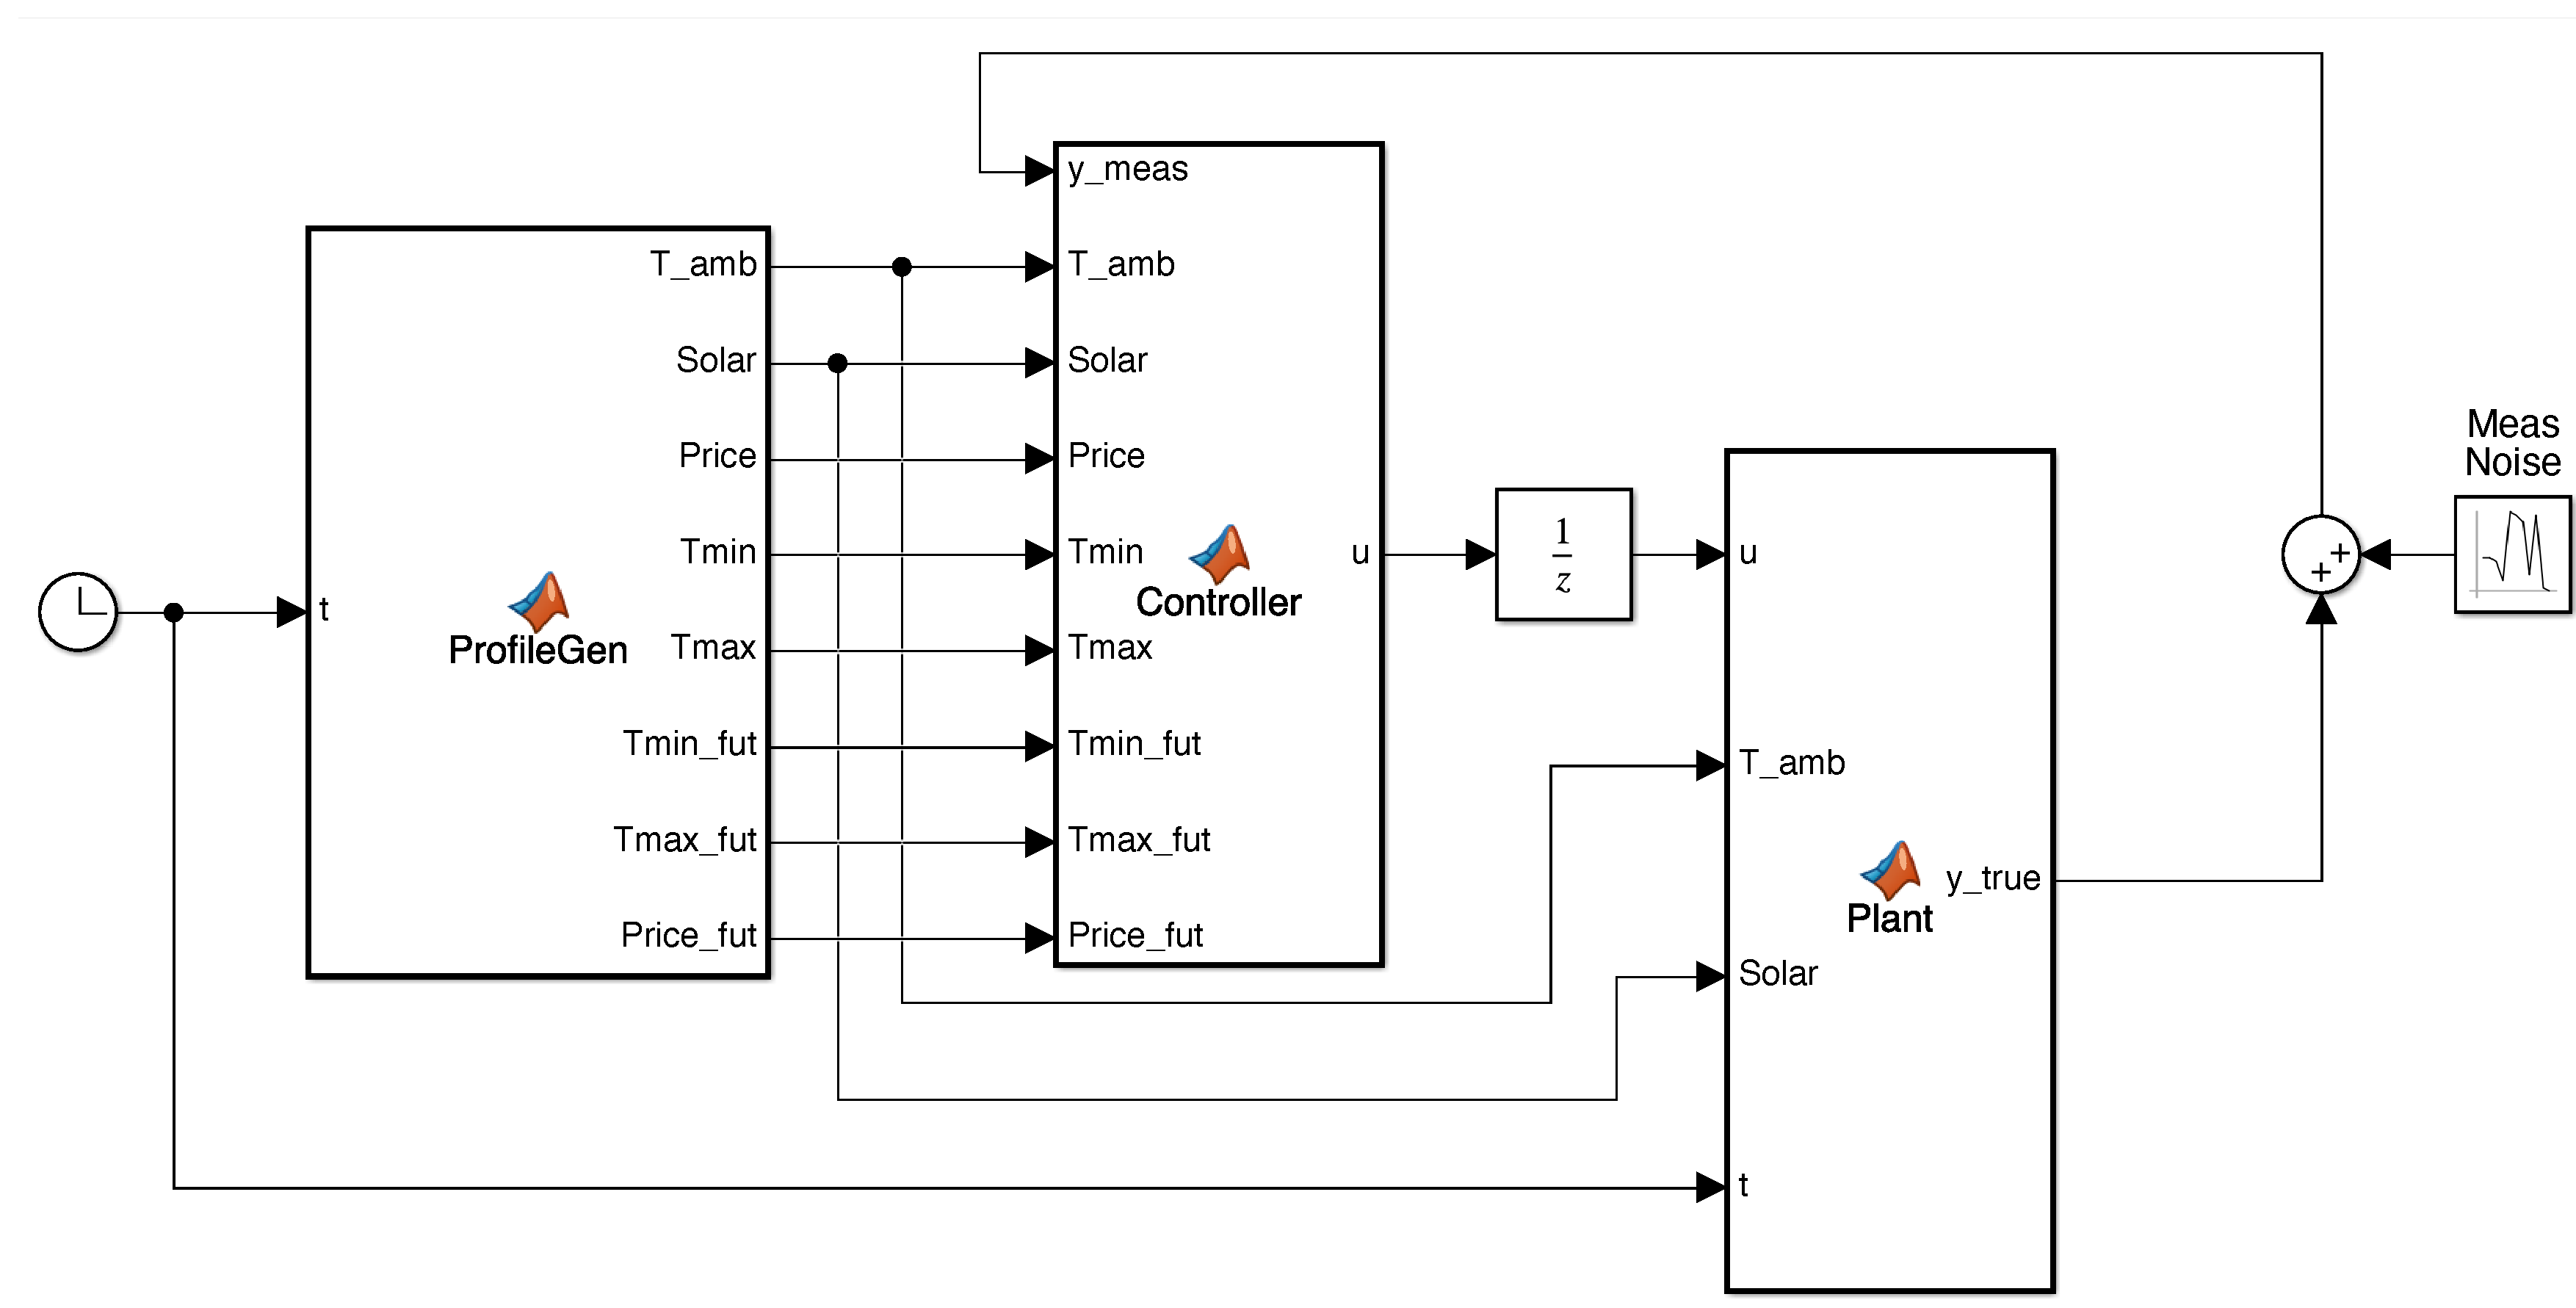
\includegraphics[width=1\linewidth]{Figures/Simulink_Building}
	\caption{HVAC Simulation using SIMULINK.}
	\label{fig:simulinkbuilding}
\end{figure}



\begin{table}[htbp]
	\centering
	\caption{Common issues and remedies for the Simulink single-zone MPC
		implementation.}
	\label{tab:troubleshoot}
	\begin{tabular}{>{\small}p{4.8cm} >{\small}p{8.8cm}}
		\toprule
		\textbf{Symptom} & \textbf{Remedy} \\
		\midrule
		\texttt{Function not found: get\_profiles} &
		Helper files are not on the MATLAB path.  Run \texttt{addpath(pwd)} or
		place all \texttt{.m} files alongside \texttt{EconomicMPC.slx}. \\[6pt]
		\texttt{Undefined function 'sdpvar'} &
		YALMIP is not installed or not on the path.  Run \texttt{yalmiptest}
		before starting Simulink. \\[6pt]
		Temperature starts from wrong value on second run &
		Persistent variables were not cleared.  Run
		\texttt{clear plant\_step mpc\_controller\_step} before pressing
		\textit{Run}. \\[6pt]
		Algebraic loop warning &
		Unit Delay block ($T_s=1800$, IC\,$=0$) is missing on the Saturation
		$\to$ Plant path.  See Section~\ref{subsec:algloop_general}. \\[6pt]
		Port dimension mismatch on \texttt{Tmin\_fut} or \texttt{Price\_fut} &
		Pre-allocation lines \texttt{Tmin\_fut = zeros(1,24)} and
		\texttt{Price\_fut = zeros(1,24)} must appear \emph{before} the
		extrinsic call in the ProfileGen wrapper. \\[6pt]
		Controller uses wrong disturbance level at night &
		Confirm the augmented model includes the correct $B_w$ column and
		that \texttt{d\_hat} (not \texttt{d\_filt}) is passed to the target
		calculator; the single-zone example does not apply exponential
		smoothing. \\[6pt]
		First step takes over 60\,s &
		Normal on low-end hardware; YALMIP is building QP matrices
		symbolically.  Do not interrupt the simulation. \\
		\bottomrule
	\end{tabular}
\end{table}


\subsection{Summary}
\label{subsec:summary}
% 

\begin{summarybox}{Simulink MPC Without the MPC Toolbox — Key Steps}
	\begin{enumerate}[noitemsep]
		\item \textbf{Helper files.}  Place all YALMIP and solver logic in
		ordinary \texttt{.m} files on the MATLAB path (Layer 2).
		\item \textbf{Persistent state.}  Store the observer state, last
		applied input, filtered disturbance, and compiled
		\texttt{optimizer} objects as \texttt{persistent} variables.
		\item \textbf{One-time compilation.}  Call
		\texttt{build\_mpc\_optimizers} on the first step only,
		guarded by \texttt{if isempty(...)}.
		\item \textbf{Wrapper blocks.}  Each Simulink MATLAB Function block
		(Layer 1) declares its helper as \texttt{coder.extrinsic},
		pre-allocates outputs, and calls the helper.
		\item \textbf{Break the algebraic loop.}  Insert a Unit Delay
		($T_s = 1800$, IC\,$= 0$) between Saturation and Plant.
		\item \textbf{Reset before each run.}  Execute
		\texttt{clear plant\_step mpc\_controller\_step} before
		pressing \textit{Run}.
	\end{enumerate}
\end{summarybox}

\section*{Chapter Summary}
\begin{itemize}
    \item Simulink integration allows MPC algorithms written in MATLAB to run inside block-diagram simulations alongside continuous-time plant models.
    \item MATLAB Function blocks embed custom MATLAB code in Simulink and interface with the solver through input and output ports.
    \item The \texttt{coder.extrinsic} directive marks functions (e.g.\ YALMIP calls) that cannot be compiled, forcing Simulink to evaluate them in the MATLAB interpreter at each time step.
    \item Persistent variables declared inside a MATLAB Function block retain their values across simulation steps, enabling stateful operations such as observer updates.
    \item The YALMIP \texttt{optimizer} object pre-compiles the QP structure once and accepts parameter updates at each call, significantly reducing per-step overhead in Simulink.
    \item A building energy MPC case study demonstrates zone temperature regulation under occupancy-driven comfort constraints and time-varying electricity pricing.
    \item The recommended simulation workflow includes model setup, controller block configuration, closed-loop wiring, and post-simulation plotting for verification.
\end{itemize}

% ─────────────────────────────────────────────────────────────
\section*{Exercises}
\label{sec:simulink_mpc_exercises}
% ─────────────────────────────────────────────────────────────

\begin{enumerate}

	\item \textbf{Persistent variables in Simulink MATLAB Function blocks.}
	In the single-zone building example, the function
	\texttt{mpc\_controller\_step} declares several \texttt{persistent}
	variables (e.g.\ the observer state~$\hat x$, the last applied
	input~$u_{k-1}$, and the compiled \texttt{optimizer} object).
	\begin{enumerate}
		\item Explain why ordinary local variables would fail to preserve
		      state across successive Simulink time steps.
		\item What would happen if the compiled \texttt{optimizer} object
		      were \emph{not} stored as a persistent variable?  Discuss the
		      implications for both correctness and computational cost.
		\item Describe the role of the \texttt{if isempty(...)} guard that
		      protects the one-time initialisation of persistent variables.
		      Why is this pattern preferred over, for example, using a
		      separate Simulink \textit{InitFcn} callback?
	\end{enumerate}

	\item \textbf{The role of \texttt{coder.extrinsic}.}
	Simulink MATLAB Function blocks are processed by MATLAB Coder, which
	requires statically typed, code-generation--compatible functions.
	\begin{enumerate}
		\item Explain why YALMIP functions (such as \texttt{sdpvar},
		      \texttt{optimize}, and \texttt{optimizer}) cannot be compiled
		      by MATLAB Coder.
		\item Describe what the \texttt{coder.extrinsic} directive does and
		      how it allows YALMIP-based helper functions to be called from
		      within a Simulink MATLAB Function block.
		\item The chapter recommends pre-allocating every output variable
		      with \texttt{zeros} \emph{before} the call to the extrinsic
		      helper.  Explain why this pre-allocation step is necessary and
		      what error would occur without it.
	\end{enumerate}

	\item \textbf{Adding a rate-of-change constraint to the building
	controller.}
	The MPC formulation in Section~\ref{sec:simulink_building} enforces box
	constraints $0 \le u_k \le 2000$\,W on the heater input but does not
	limit how quickly the input may change between consecutive steps.
	Suppose you wish to add the constraint
	$|\Delta u_k| = |u_k - u_{k-1}| \le \Delta u_{\max}$
	with $\Delta u_{\max} = 500$\,W.
	\begin{enumerate}
		\item Describe which file(s) in the two-layer architecture you would
		      need to modify and what YALMIP constraints you would add inside
		      the prediction-horizon loop.
		\item Explain why the persistent variable \texttt{u\_prev} (the last
		      applied input) must be passed as a \emph{parameter} to the
		      \texttt{optimizer} object so that the rate constraint can
		      reference the transition from $u_{k-1}$ to the first predicted
		      input $u_0$.
		\item Discuss qualitatively how adding a tight rate-of-change limit
		      would affect the closed-loop temperature response during
		      morning warm-up, when a large step in heating power would
		      otherwise be applied.
	\end{enumerate}

	\item \textbf{The algebraic-loop problem and the Unit Delay solution.}
	Section~\ref{sec:simulink_general} explains that a direct connection
	from the MPC controller output to the plant input, and from the plant
	output back to the controller, creates an algebraic loop.
	\begin{enumerate}
		\item Draw a simplified signal-flow diagram showing the loop and
		      explain, in your own words, why Simulink cannot determine a
		      consistent set of signals at a single time step when the loop
		      is present.
		\item Explain how inserting a Unit Delay block (with sample time
		      $T_s = 1800$\,s and initial condition $u_0 = 0$) breaks the
		      algebraic loop.  What is the physical interpretation of
		      applying the control action one sample period later?
		\item In practice, MPC already computes the control move for the
		      \emph{current} time step.  Argue whether the one-step delay
		      introduced by the Unit Delay block materially degrades
		      closed-loop performance for a slowly varying building thermal
		      system with a 30-minute sample time.
	\end{enumerate}

	\item \textbf{Designing a Simulink MPC architecture for a DC motor.}
	Consider a DC motor whose angular velocity $\omega$ is governed by the
	simplified continuous-time transfer function
	\[
		G(s) = \frac{\omega(s)}{V(s)} = \frac{K}{\tau s + 1},
	\]
	where $V$ is the armature voltage, $K = 10$\,rad\,s$^{-1}$\,V$^{-1}$,
	and $\tau = 0.1$\,s.  The input is subject to
	$0 \le V \le 24$\,V, and the objective is to track a reference speed
	$\omega_{\mathrm{ref}}(t)$.
	\begin{enumerate}
		\item Discretise the plant with a suitable sample time (justify your
		      choice) and write down the resulting state-space matrices
		      $A_d$, $B_d$, $C_d$, $D_d$.
		\item Sketch a Simulink block diagram following the two-layer
		      architecture from this chapter.  Label each block
		      (\textit{Reference Generator}, \textit{MPC Controller},
		      \textit{DC Motor Plant}, \textit{Scope / To Workspace}) and
		      indicate where a Unit Delay block should be placed.
		\item List the persistent variables you would declare inside the
		      \texttt{mpc\_controller\_step} function for this system.
		      Identify any differences from the building-heating case study
		      (e.g.\ is a disturbance observer still needed?).
		\item Briefly discuss how the much shorter time constant of the DC
		      motor ($\tau = 0.1$\,s) compared with the building
		      ($\tau \approx 10^4$\,s) affects the choice of prediction
		      horizon and the computational burden of solving the QP at each
		      step.
	\end{enumerate}

\end{enumerate}